% 3.1 — fuente: dump del MySQL de producción del portal anterior (documento/referencias/isidump.sql, 2026-09-17), consultas SQL
% sobre una copia local; cifras y consultas resumidas en documento/12-necesidades-cap3.md (H1–H9) y documento/16-hallazgos-cap3.md.
% Las planillas Excel de control todavía no están disponibles: cuando lleguen se agregan a 3.1.1 y se recalculan las cifras.
\subsection{ANÁLISIS DE DATOS HISTÓRICOS}

Este análisis responde al segundo objetivo específico: determinar, con los datos y no con supuestos, si el histórico permite construir los tres casos de uso del módulo predictivo, con qué variables y sobre cuántos casos. Se realizó sobre una copia completa de la base de datos de producción del portal anterior, exportada en septiembre de 2026 y cargada en un servidor MySQL local, sin conexión con el sistema en operación. Las cifras de esta sección provienen de consultas SQL sobre esa copia; el pipeline de la sección 3.4 las reproduce con DuckDB y Polars. Las planillas Excel de control de proyectos que la empresa lleva fuera del sistema no estaban disponibles al cierre de este análisis, por lo que las cifras corresponden solo a la base de datos del portal.

\subsubsection{EXPLORACIÓN Y CARACTERIZACIÓN DE LAS FUENTES DE DATOS}

La base del portal contiene 163 tablas con datos. La mayoría son catálogos, permisos y tablas de recursos humanos; estas últimas, con remuneraciones y datos personales, se excluyeron del análisis desde el inicio (RNF-03). La tabla~\ref{tab:fuentes-historico} resume las tablas de la base que describen la ejecución de los proyectos. No se encontró una tabla de certificaciones como tal: las certificaciones son ítems del flujo de caja de cada proyecto, identificados por su rubro, con fecha planificada y fecha real.

\begin{tabla}[H]
  \centering
  \caption{Tablas del portal anterior usadas en el análisis}\label{tab:fuentes-historico}
  \small
  \begin{tblr}{colspec={X[1.04,l] X[1.82,l] X[0.44,r] X[0.7,l]}}
    \textbf{Tabla} & \textbf{Contenido} & \textbf{Filas} & \textbf{Período} \\
    \texttt{act\_proyecto} & Maestro de centros de costo: fechas, plazo, monto de la orden de compra, presupuesto de costo por rubro, horas planificadas, margen proyectado & 292 & 2003--2026 \\
    \texttt{adicionales} & Ampliaciones de alcance con su monto y costo presupuestado & 237 & 2005--2020 \\
    \texttt{gpre} & Flujo de caja vigente por ítem; las certificaciones son los rubros \texttt{WI001} (orden de compra) y \texttt{WA001} (adicionales) & 10\,872 & 2008--2027 \\
    \texttt{gprepublicadomensual} & Foto mensual del flujo de caja publicado & 170\,225 & 2013--2020 \\
    \texttt{gpreeventos} & Registro de cambios al flujo de caja & 47\,896 & 2013--2020 \\
    \texttt{gpdir} & Asientos contables por centro de costo: débito como costo y crédito como ingreso & 81\,307 & 2008--2025 \\
    \texttt{horas}, \texttt{horasctroctos} & Horas diarias por persona y su asignación a centros de costo & 310\,137 & 2005--2024 \\
    \texttt{rq} & Requisiciones de compra & 6\,165 & 2006--2026 \\
    \texttt{viaticos} & Pedidos de viáticos & 3\,713 & 2011--2026 \\
    \texttt{propuestas} & Oportunidades comerciales, con el sector industrial & 844 & 2013--2026 \\
  \end{tblr}
  \fuente{Elaboración propia, 2026, en base a la base de datos del portal anterior.}
\end{tabla}

El universo de análisis son los centros de costo cerrados de tipo proyecto (prefijos \texttt{O} y \texttt{C}) y servicio (prefijo \texttt{S}): 248 centros de costo, 175 de proyecto u operación, 57 de servicio y 16 de consultoría, con fechas de inicio entre 2003 y 2026. La figura~\ref{fig:proyectos-anio} muestra su distribución por año de inicio y, para cada año, cuántos tienen un flujo de caja con certificaciones. El hallazgo central es que el flujo de caja del portal se usó para planificar y registrar certificaciones solo entre 2010 y 2018: antes de 2010 casi no hay certificaciones registradas, y a partir de 2019 los proyectos siguen teniendo costos contables, pero no certificaciones.

\begin{figure}[H]
\centering
\caption{Centros de costo cerrados por año de inicio}\label{fig:proyectos-anio}
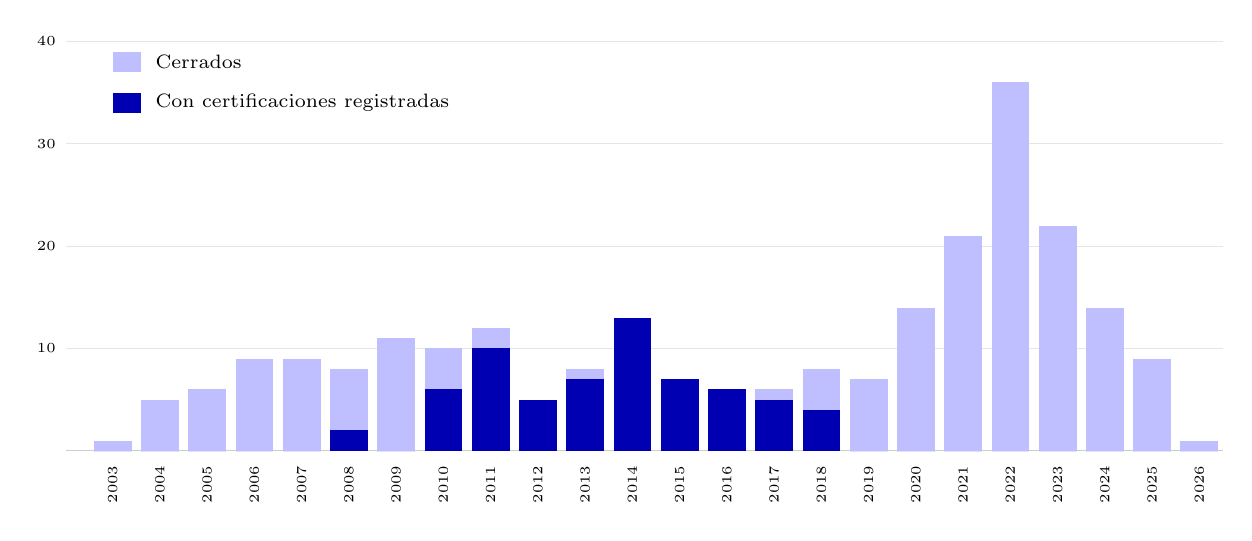
\begin{tikzpicture}[x=0.6cm, y=0.13cm]
  \draw[gray!40] (0,0) -- (24.5,0);
  \foreach \v in {10,20,30,40} {
    \draw[gray!20] (0,\v) -- (24.5,\v);
    \node[font=\tiny, anchor=east] at (0,\v) {\v};
  }
  \foreach \i/\y/\c/\k in {1/2003/1/0, 2/2004/5/0, 3/2005/6/0, 4/2006/9/0, 5/2007/9/0, 6/2008/8/2, 7/2009/11/0, 8/2010/10/6, 9/2011/12/10, 10/2012/5/5, 11/2013/8/7, 12/2014/13/13, 13/2015/7/7, 14/2016/6/6, 15/2017/6/5, 16/2018/8/4, 17/2019/7/0, 18/2020/14/0, 19/2021/21/0, 20/2022/36/0, 21/2023/22/0, 22/2024/14/0, 23/2025/9/0, 24/2026/1/0} {
    \fill[blue!25] (\i-0.4,0) rectangle (\i+0.4,\c);
    \fill[blue!70!black] (\i-0.4,0) rectangle (\i+0.4,\k);
    \node[font=\tiny, rotate=90, anchor=east] at (\i,-0.5) {\y};
  }
  \fill[blue!25] (1,37) rectangle (1.6,39); \node[font=\scriptsize, anchor=west] at (1.7,38) {Cerrados};
  \fill[blue!70!black] (1,33) rectangle (1.6,35); \node[font=\scriptsize, anchor=west] at (1.7,34) {Con certificaciones registradas};
\end{tikzpicture}
\fuente{Elaboración propia, 2026, en base a la base de datos del portal anterior.}
\end{figure}

La calidad de los datos se evaluó con las dimensiones de la sección 2.3, respecto de su uso en el módulo predictivo (cuadro~\ref{tab:calidad-historico}). Dos defectos condicionan el diseño. El primero es que el flujo de caja sobrescribe la fecha planificada de cada certificación cuando se replanifica, de modo que comparar la fecha planificada vigente con la real no mide ningún desvío; la fecha original solo puede recuperarse de las fotos mensuales, que existen desde julio de 2013. El segundo es que la fecha de cierre de los proyectos es administrativa: ocho fechas concentran cinco o más cierres cada una, y seis proyectos figuran cerrados antes de su inicio. Tampoco se registraron causas de desviación: las columnas previstas para la causa y la mitigación están vacías, lo que descarta la hipótesis planteada en la sección 1.4 de que las causas documentadas pudieran usarse como parte del conjunto de datos.

\begin{table}[H]
  \centering
  \caption{Calidad del histórico del portal anterior por dimensión}\label{tab:calidad-historico}
  \small
  \begin{tblr}{colspec={X[0.49,l] X[1.63,l] X[0.88,l]}}
    \textbf{Dimensión} & \textbf{Hallazgo} & \textbf{Efecto en el módulo} \\
    Exactitud & Fecha planificada de certificación sobrescrita al replanificar; fecha de cierre administrativa; en 28 de 60 proyectos la última certificación real coincide exactamente con la planificada original & Etiquetas de desvío y de retraso \\
    Completitud & Sin causas de desviación; certificaciones solo en 2010--2018; antes de 2020, solo entre un cuarto y un tercio de las horas cargadas pueden asignarse a un centro de costo; sector industrial registrado solo desde 2020 & Tamaño del conjunto y variables disponibles \\
    Consistencia & El ingreso contable convertido a dólares concilia con la orden de compra más adicionales (diferencia menor al 15\,\%) en 113 proyectos; desde 2020 el rubro contable de los asientos está vacío en la mayoría de los casos & Etiqueta de sobrecosto \\
    Unicidad & Siete códigos de centro de costo aparecen dos veces en el maestro de proyectos & Deduplicación en Silver \\
    Validez & Tipo de cambio igual a uno en casi todos los asientos de 2008 a 2010 y en la mayoría de los de 2012, con moneda ambigua; plazos de ejecución de 1 a 7 días en proyectos de meses; cierre anterior al inicio; texto con codificación dañada & Filtros y variables excluidas \\
    Oportunidad & No evaluada: el portal no registra cuándo se cargó cada dato respecto del evento & --- \\
  \end{tblr}
  \fuente{Elaboración propia, 2026, en base a la base de datos del portal anterior y de la sección 2.3.}
\end{table}

\subsubsection{IDENTIFICACIÓN DE VARIABLES PREDICTORAS}

Una variable candidata debe cumplir dos condiciones: estar disponible en el histórico con completitud suficiente y tener equivalente en el ERP nuevo, donde se realiza la inferencia. La tabla~\ref{tab:variables-candidatas} evalúa las candidatas sobre los 75 centros de costo cerrados que iniciaron entre 2010 y 2018, el período en que existen las etiquetas.

\begin{tabla}[H]
  \centering
  \caption{Variables predictoras candidatas}\label{tab:variables-candidatas}
  \footnotesize
  \begin{tblr}{colspec={X[1.19,l] X[0.62,r] X[0.97,l] X[1.23,l]}}
    \textbf{Variable} & \textbf{Completitud 2010--2018} & \textbf{Equivalente en el ERP nuevo} & \textbf{Decisión} \\
    Monto vendido y presupuesto de costo por bolsa & 97--99\,\% & Líneas de presupuesto de línea base & Se usa \\
    Horas planificadas & 94\,\% & Horas de la bolsa de servicios & Se usa \\
    Margen bruto proyectado & 87\,\% & Derivable del vendido & Se usa \\
    Ampliaciones de alcance & 61\,\% con adicionales & Crecimiento del vendido desde la línea base inicial & Se usa como crecimiento del vendido \\
    Replanificaciones del flujo de caja & 94\,\% & Bitácora del presupuesto & Se usa \\
    Costo ejecutado acumulado & 100\,\% (83\,\% concilia) & Ejecutado del presupuesto & Se usa \\
    Certificado acumulado frente a planificado & 84\,\% & Certificaciones & Se usa \\
    Requisiciones y viáticos & 79 y 66\,\% & Órdenes de compra y rendiciones & Se usa; ausencia equivale a cero \\
    Horas cargadas & 99\,\% con horas, cobertura parcial & Horas aprobadas & Se usa con cautela; se evalúa su aporte \\
    Tipo de centro de costo & 100\,\% & Tipo de centro de costo & Se usa \\
    Plazo de ejecución registrado & 100\,\% & Fechas de vigencia & Se descarta: valores no comparables \\
    Sector industrial & 0\,\% & Mercado de la propuesta & Se descarta en el entrenamiento \\
    Cliente & No resoluble & Cliente & Se descarta: los identificadores no existen en las tablas de clientes \\
    Avance físico & No existe & No existe & Se descarta \\
  \end{tblr}
  \fuente{Elaboración propia, 2026, en base a la base de datos del portal anterior y del esquema del ERP nuevo.}
\end{tabla}

Las variables retenidas describen el proyecto por su tamaño, la composición de su presupuesto, la estabilidad de su plan y el ritmo de su ejecución económica. Ninguna mide el avance físico, que el portal no registraba y el ERP nuevo tampoco define (sección 3.2); el avance se aproxima con el tiempo transcurrido, el costo ejecutado y lo certificado frente a lo planificado. Como las variables se calculan a una fecha de corte (sección 3.4), cada una se reconstruye solo con los registros fechados hasta ese corte.

\subsubsection{DEFINICIÓN DE CASOS DE USO PREDICTIVOS}

Los tres casos de uso se definen con reglas de etiquetado explícitas, aplicables por igual al histórico y al ERP nuevo. Los umbrales siguen el semáforo del ERP: una desviación desfavorable de hasta 5\,\% es verde, de hasta 10\,\% amarilla y mayor, roja (REQ~12.11); para las certificaciones, el requerimiento de la empresa fija en 10\,\% el desvío que exige causa y mitigación (REQ~13.9). La tabla~\ref{tab:casos-uso} resume el resultado.

\paragraph{Desviación en certificaciones}

La unidad es la certificación. Se considera desviada si se certificó después de su fecha planificada original por más del 10\,\% del plazo planificado del proyecto, o por un monto inferior en más del 10\,\% al planificado originalmente. El plazo planificado es el tiempo entre el inicio del proyecto y su última certificación planificada original. Con la fecha original tomada de las fotos mensuales, se obtienen 831 certificaciones con fecha real de 65 proyectos, de las cuales 134 (16\,\%) están desviadas. La cifra está sesgada a la baja para los proyectos iniciados antes de julio de 2013, cuyo plan ya podía estar modificado cuando se tomó la primera foto: entre los 42 proyectos iniciados después, 113 de 389 certificaciones (29\,\%) están desviadas.

\paragraph{Sobrecosto}

La unidad es el proyecto. El sobrecosto es el costo ejecutado al cierre respecto del vendido, en porcentaje. En el histórico, el costo ejecutado se toma de los asientos contables convertidos a dólares, y el vendido, del presupuesto de costo más los adicionales. Solo se usan los proyectos cuyo ingreso contable concilia con la orden de compra más adicionales, como control de que la conversión de moneda es correcta: 113 proyectos. De ellos, 61 cerraron por debajo del vendido, 13 lo superaron hasta en un 10\,\% y 39 en más del 10\,\%. Diez superan el 100\,\%, valores que se revisan como posibles errores de registro antes del entrenamiento.

\paragraph{Retraso en la fecha de cierre}

La unidad es el proyecto. Como la fecha de cierre registrada es administrativa, el fin real se toma de la última certificación real y el fin planificado, de la última certificación planificada en la primera foto mensual. El retraso se expresa como porcentaje del plazo planificado. Con proyectos de al menos treinta días de plazo planificado se obtienen 60 casos: 17 (28\,\%) con retraso mayor al 10\,\%, 6 con retraso de hasta 10\,\% y 37 terminados en plazo o antes. En 28 de ellos la fecha real coincide exactamente con la planificada, lo que puede reflejar un plazo cumplido o una fecha real cargada igual a la planificada; esa ambigüedad se trata como limitación.

\begin{tabla}[H]
  \centering
  \caption{Casos de uso predictivos y tamaño de sus conjuntos de datos}\label{tab:casos-uso}
  \small
  \begin{tblr}{colspec={X[1.1,l] X[0.76,l] X[0.93,l] X[1.1,l] X[1.1,l]}}
    \textbf{Caso de uso} & \textbf{Unidad} & \textbf{Tipo de problema} & \textbf{Casos con etiqueta} & \textbf{Casos desfavorables} \\
    Desviación en certificaciones & Certificación & Clasificación & 831 de 65 proyectos & 134 desviadas (16\,\%) \\
    Sobrecosto & Proyecto & Regresión & 113 & 39 sobre 10\,\% (35\,\%) \\
    Retraso en la fecha de cierre & Proyecto & Regresión & 60 & 17 sobre 10\,\% (28\,\%) \\
  \end{tblr}
  \fuente{Elaboración propia, 2026, en base a la base de datos del portal anterior.}
\end{tabla}

Los tamaños confirman la advertencia de la sección 2.2: el histórico reúne cientos de casos para las certificaciones y apenas decenas de proyectos para los otros dos casos de uso. Esto justifica dos decisiones del diseño. La primera es modelar la desviación en certificaciones por certificación y no por proyecto, porque es la única unidad con volumen suficiente. La segunda es observar cada proyecto en varias fechas de corte y validar agrupando por proyecto (sección 3.4), para aprovechar los pocos proyectos sin sobrestimar el desempeño. El tamaño reducido de los conjuntos de sobrecosto y retraso es la principal limitación del módulo predictivo; las planillas de control, si cubren los proyectos posteriores a 2018, son la vía para ampliarlos.
